In this section, we present Madeus' performance model. Its goal is,
given a Madeus assembly to be deployed and the execution time of all the
transitions of all the components in an assembly, to predict the total
execution time of the deployment.
%
Intuitively, we automatically model the execution flow of a Madeus
assembly based on Madeus' formal semantics. This is done by generating a
dependency graph representations of the execution flow of each Madeus
component in the assembly and connecting them together according to their
dependencies (the connections between their ports). We then add a
\emph{source} vertex connected to the vertices representing the beginning of
the execution of each component, as well as a \emph{sink} vertex to which
are connected the vertices representing the end of the execution of each
component.
%
We obtain a dependency graph representing the execution of the whole
assembly. By weighting the arcs corresponding to the transitions with
these transitions' individual execution time (and the other ones with 0),
we can find the total execution time of the assembly by finding the longest
path from the \emph{source} vertex to the \emph{sink} vertex.

% By generating a graph modelling the execution flow of a Madeus assembly,
% capturing both intra-component and inter-component dependencies, we
% reduce this problem to finding the longest path in a DAG.

\subsection{Notations}

Recall that given a component, we denote its set of places $\Pi$ and its
set of transitions $\Theta$. In the following, we will consider for the
sake of simplicity that the transitions go directly from a place to
another place instead of from an output dock to an input dock.
Hence, $\Theta$ is a multiset which elements are couples of places. We
can obtain the place corresponding to each dock by using the $place$
function of the component.

In order to predict the total deployment time, we need to know the
execution time of each individual transition. In the following, we
consider the \emph{time function} $time\,:\,\Theta\rightarrow\mathbb{R}^{+}$
associating a running time to each transition (taken as input).

We also consider the following two functions:
\begin{itemize}
\item the \emph{group entrance function} $g_{in}\,:\,G\rightarrow\mathcal{P}\left(\Pi\right)\,g\mapsto\left\{ \pi\,\mid\,\pi\in g\land\exists\pi_{b}\,:\,\left(\pi_{b}\not\in g\land\left(\pi_{b},\pi\right)\in\Theta\right)\right\} $
(the result of $g_{in}$ is called the set of \emph{entrance places}
of the group)
\item the \emph{group exit function} $g_{out}\,:\,G\rightarrow\mathcal{P}\left(\Pi\right)g\mapsto\left\{ \pi\,\mid\,\pi\in g\land\exists\pi_{a}\,:\,\left(\pi_{a}\not\in g\land\left(\pi,\pi_{a}\right)\in\Theta\right)\right\} $
(the result of $g_{out}$ is called the set of \emph{exit places}
of the group)
\end{itemize}

Recall that an assembly is a tuple $\left(C,L_{P},L_{D},ebl\right)$. In
the following, we consider that
$C=\bigcup_{i=1}^{n}\left\{ \left(\Pi_{i}\dots,\left(B_{D_{p}}\right)_{i}\right)\right\} $.
For each notation $X$ specific to a component, we denote $X_{all}$ the
union (in the case of an assembly) or the extension (in the case of
a function) for all components. For instance:
\begin{itemize}
\item $\Pi_{all}=\bigcup_{i=1}^{n}\Pi_{i}$ (set of all \emph{places} in
the assembly)
\item $\left(time\right)_{all}\,:\,\Theta_{all}\rightarrow\mathbb{R}^{+}$
(function giving the \emph{running time} of each transition) with:
$\left(time\right)_{all}\left(x\right)=\left(time\right)_{i}\left(x\right)$
if $x\in\Theta_{i}$ 
\end{itemize}
The execution flow graph is an oriented weighted graph \emph{$\left(V,A\right)$}
where $V$ is the set of vertices and $A$ is the multiset of weighted
arcs with elements in $V\times V\times\mathbb{R}^{+}$. We define
$V$ an $A$ in the following.

\subsection{Vertices}

For each place, we associate two vertices: one representing the place
itself and one representing the action of a token leaving the place.
Figure~\ref{fig:place_graph} depicts the transformation of one place
\emph{running} to a dependency graph.
\[
V_{\Pi}=\bigcup_{\pi\in\Pi_{all}}\left\{ v_\pi^\text{place},v_\pi^\text{leaving}\right\} 
\]

For each transition, we associate two vertices: one representing the
beginning of the transition and one representing its end.
Figure~\ref{fig:transition_graph} depicts the transformation of three
transitions \emph{t1}, \emph{t2} and \emph{t3} to a dependency graph.
\[
V_{\Theta}=\bigcup_{\theta\in\Theta_{all}}\left\{ v_\theta^\text{beginning},v_\theta^\text{end}\right\} 
\]

For each data (use or provide) port we associate one vertex representing
its activation.
Figure~\ref{fig:data_ports_graph} depicts the transformation of one
data provide port \emph{dp} and one data use port \emph{du}.
\[
V_{data}=\bigcup_{u\in\left(D_{u}\right)_{all}\cup\left(D_{p}\right)_{all}}\left\{ v_u^\text{start}\right\} 
\]

For each service (use or provide) port we associate two vertices:
one representing its activation and one its deactivation.
Figure~\ref{fig:service_ports_graph} depicts the transformation of one
service provide port \emph{dp} and one service use port \emph{du}.
\[
V_{service}=\bigcup_{p\in\left(P_{u}\right)_{all}\cup\left(P_{p}\right)_{all}}\left\{v_p^\text{start},v_p^\text{stop}\right\} 
\]

Finally, we define $V$ as the union of all these, plus one source
and one sink vertices. 
\[
V=V_{\Pi}\cup V_{\Theta}\cup V_{data}\cup V_{service}\cup\left\{ v^\text{source},v^\text{sink}\right\} 
\]


\subsection{Arcs}

In the performance graph, arcs represent time constraints: the event represented
by the destination vertex must happen after the one represented by the source
vertex, at least $w$ seconds apart where $w$ is the weight of the arc. In
practice, the weight of all of the arcs except those corresponding to the
transitions is 0. The weights of the latter are the execution times of the
transitions.

For each place $\pi$ we associate one arc going from $v_\pi^\text{place}$ to
$v_\pi^\text{leaving}$. This represents the fact that a token may leave $\pi$
only after it has entered it.
Figure~\ref{fig:place_graph} depicts the transformation of one place
\emph{running} to a dependency graph.
\[
A_{\Pi}=\bigcup_{\pi\in\Pi_{all}}\left\{ \left(v_\pi^\text{place},v_\pi^\text{leaving},0\right)\right\} 
\]

\begin{figure}[h]
  \subfloat[Concerto assembly]{%
    \begin{minipage}[c]{0.5\columnwidth}%
      \centering
      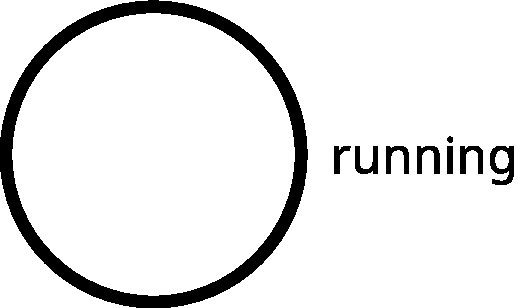
\includegraphics[scale=0.2]{images/perf_place.pdf}
    \end{minipage}
  }
  \subfloat[Dependency graph]{%
    \begin{minipage}[c]{0.5\columnwidth}%
      \centering
      \begin{tikzpicture}[node distance=1.7cm]
        \node (leaving) [leaving] {$v_\text{running}^\text{leaving}$};
        \node (place) [place, below of=leaving] {$v_\text{running}^\text{place}$};
        \draw [arrow] (place) -- (leaving) node[midway, right] {$0$};
      \end{tikzpicture}
    \end{minipage}
  }
  \caption{Vertices and arcs for a place}
  \label{fig:place_graph}
\end{figure}

For each transition $\theta$ going from $\pi_s$ to $\pi_d$, we associate
three arcs. The first between $v_\theta^\text{beginning}$ and $v_\theta^\text{end}$
represents the fact that the end of $\theta$ happens at the time of the
start of $\theta$ plus its duration. The second between $v_{\pi_{s}}^\text{leaving}$
and $v_\theta^\text{beginning}$ represents the fact that $\theta$ may only
happen after a token leaved $\pi_s$. The third one between $v_\theta^\text{end}$ and
$v_{\pi_{d}}^\text{place}$ represents the fact that a token may enter $\pi_d$ only
after $\theta$ has finished.
Figure~\ref{fig:transition_graph} depicts the transformation of three
transitions \emph{t1}, \emph{t2} and \emph{t3} to a dependency graph.
\begin{align*}
A_{\Theta}=\bigcup_{\theta=\left(\pi_{s},\pi_{d}\right)\in\Theta_{all}} & \left\{ \left(v_\theta^\text{beginning},v_\theta^\text{end},time_{all}\left(\theta\right)\right),\right.\\
 & \left(v_{\pi_{s}}^\text{leaving},v_\theta^\text{beginning},0\right),\\
 & \left. \left(v_\theta^\text{end},v_{\pi_{d}}^\text{place},0\right)\right\}
\end{align*}

\begin{figure*}[h]
  \subfloat[Concerto assembly]{%
    \begin{minipage}[c]{0.8\columnwidth}%
      \centering
      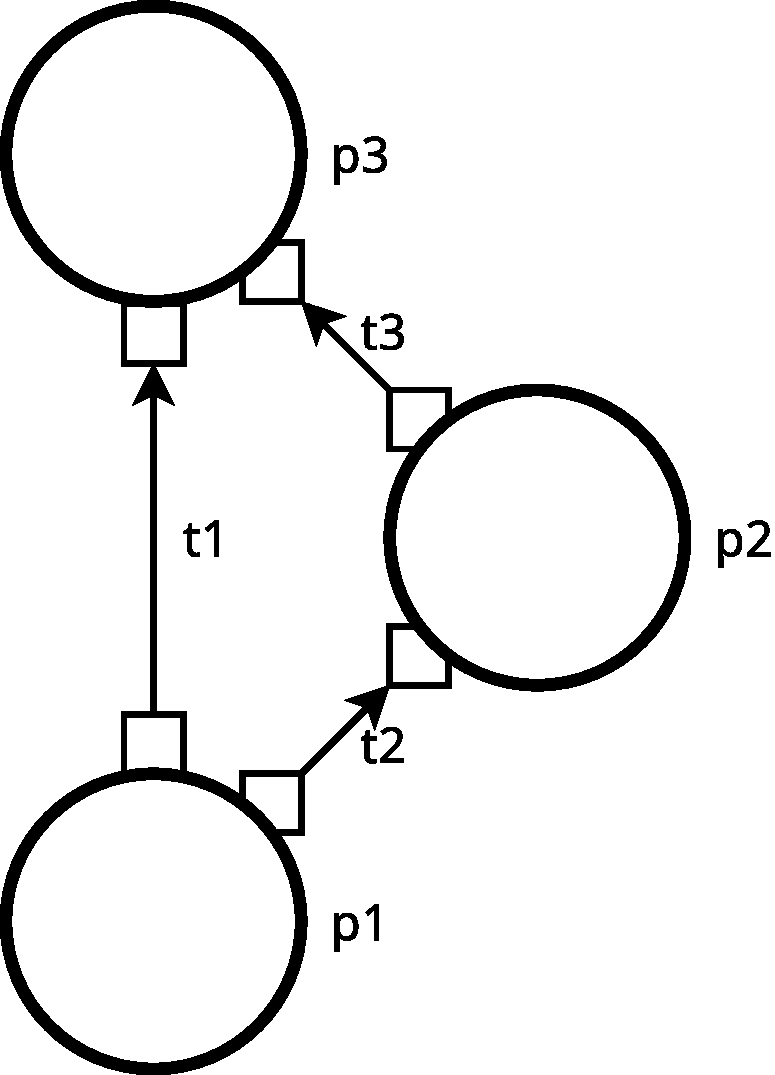
\includegraphics[scale=0.2]{images/perf_transition.pdf}
    \end{minipage}
  }
  \hfill
  \subfloat[Dependency graph]{%
    \begin{minipage}[c]{1.2\columnwidth}%
      \centering
      \begin{tikzpicture}[node distance=1.7cm]
        \node (p3l) [leaving] {$v_\text{p3}^\text{leaving}$};
        \node (p3) [place, below of=p3l] {$v_\text{p3}^\text{place}$};
        \node (t1e) [end, below of=p3] {$v_\text{t1}^\text{end}$};
        \node (t1) [beginning, below of=t1e] {$v_\text{t1}^\text{beginning}$};
        \node (p1l) [leaving, below of=t1] {$v_\text{p1}^\text{leaving}$};
        \node (p1) [place, below of=p1l] {$v_\text{p1}^\text{place}$};
        \node (t2) [beginning, right of=p1l, xshift=1.8cm] {$v_\text{t2}^\text{beginning}$};
        \node (t2e) [end, right of=t2, xshift=1.8cm] {$v_\text{t2}^\text{end}$};
        \node (p2) [place, above of=t2e] {$v_\text{p2}^\text{place}$};
        \node (p2l) [leaving, above of=p2] {$v_\text{p2}^\text{leaving}$};
        \node (t3) [beginning, above of=p2l] {$v_\text{t3}^\text{beginning}$};
        \node (t3e) [end, right of=p3, xshift=1.8cm] {$v_\text{t3}^\text{end}$};
        \draw [arrow] (p3) -- (p3l) node[midway, right] {$0$};
        \draw [arrow] (p2) -- (p2l) node[midway, right] {$0$};
        \draw [arrow] (p1) -- (p1l) node[midway, right] {$0$};
        \draw [arrow] (t3) -- (t3e) node[midway, above] {$time(\text{t3})$};
        \draw [arrow] (t2) -- (t2e) node[midway, below] {$time(\text{t2})$};
        \draw [arrow] (t1) -- (t1e) node[midway, right] {$time(\text{t1})$};
        \draw [arrow] (p1l) -- (t1) node[midway, right] {$0$};
        \draw [arrow] (p1l) -- (t2) node[midway, below] {$0$};
        \draw [arrow] (p2l) -- (t3) node[midway, right] {$0$};
        \draw [arrow] (t1e) -- (p3) node[midway, right] {$0$};
        \draw [arrow] (t2e) -- (p2) node[midway, right] {$0$};
        \draw [arrow] (t3e) -- (p3) node[midway, above] {$0$};
      \end{tikzpicture}
    \end{minipage}
  }
  \caption{Vertices and arcs for transitions}
  \label{fig:transition_graph}
\end{figure*}

For each binding between a data use port $p$ and a transition $\theta$ we
associate one arc going from $v_p^\text{start}$ to $v_\theta^\text{beginning}$.
This represents the fact that the transition may only begin after the port has
received data.
Figure~\ref{fig:data_ports_graph} depicts the transformation of a
data use port \emph{du} bound to transition \emph{c2t}.
\[
A_{D_{u}}=\bigcup_{\left(p,\theta\right)\in\left(B_{D_{u}}\right)_{all}}\left\{ \left(v_p^\text{start},v_\theta^\text{beginning},0\right)\right\} 
\]

For each binding between a data provide port $p$ and a place $\pi$ we associate
one arc going from $v_\pi^\text{place}$ to $v_p^\text{start}$. This represents
the fact that the data may only be provided after the place $\pi$ has been
reached by a token.
Figure~\ref{fig:data_ports_graph} depicts the transformation of a
data provide port \emph{dp} bound to place \emph{c1p}.
\[
A_{D_{p}}=\bigcup_{\left(p,\pi\right)\in\left(B_{D_{p}}\right)_{all}}\left\{ \left(v_\pi^\text{place},v_p^\text{start},0\right)\right\} 
\]

For each binding between a service use port $p$ and a transition $\theta$ we
associate two arcs. The first from $v_p^\text{start}$ to
$v_\theta^\text{beginning}$ represents the fact that $\theta$ can only start
once the service is provided. The second from $v_\theta^\text{end}$ to
$v_p^\text{stop}$ represents the fact that the service may only stop being
provided after $\theta$ has finished.
Figure~\ref{fig:service_ports_graph} depicts the transformation of a
service use port \emph{su} bound to transition \emph{c2t}.
\[
A_{P_{u}}=\bigcup_{\left(p,\theta\right)\in\left(B_{P_{u}}\right)_{all}}\left\{ \left(v_p^\text{start},v_\theta^\text{beginning},0\right),\left(v_\theta^\text{end},v_p^\text{stop},0\right)\right\} 
\]

For each binding between a service provide port $p$ and a group $g$ we
associate two sets of arcs. The first set of transitions going from
$v_\pi^\text{place}$ to $v_p^\text{start}$ for each place $\pi$ in the
entrance of $g$ represents the fact that a token must enter the group
before the service becomes active. The second set of transitions going
from $v_p^\text{stop}$ to $v_\pi^\text{leaving}$ for each place
$\pi$ in the exit of $g$ represents the fact that the service must not
be in use anymore before all tokens can leave the group.
Figure~\ref{fig:service_ports_graph} depicts the transformation of a
service provide port \emph{sp} bound to the group containing places
\emph{c1p1} and \emph{c1p2}. Note that \emph{c1p1} is the only entry
place of the group and \emph{c1p2} is the only exit place.
\begin{align*}
A_{P_{p}}=\bigcup_{\left(p,g\right)\in\left(B_{P_{p}}\right)_{all}} & \left( \bigcup_{\pi\in\left(g_{in}\right)_{all}\left(g\right)}\left\{ \left(v_\pi^\text{place},v_p^\text{start},0\right)\right\} \cup \right. \\
 & \left. \bigcup_{\pi\in\left(g_{out}\right)_{all}\left(g\right)}\left\{ \left(v_p^\text{stop},v_\pi^\text{leaving},0\right)\right\} \right)
\end{align*}

For each connection between data provide port $p$ and data use port $u$
in the assembly, we associate one arc going from $v_p^\text{start}$ to
$v_u^\text{start}$. This represents the fact that the data may only be
used after it has been provided.
Figure~\ref{fig:data_ports_graph} depicts the transformation of a
connection between data provide port \emph{dp} and data use port
\emph{du}.
\[
A_{L_{D}}=\bigcup_{\left(p,u\right)\in L_{D}}\left\{ \left(v_p^\text{start},v_u^\text{start},0\right)\right\} 
\]

\begin{figure*}[h]
  \subfloat[Concerto assembly]{%
    \begin{minipage}[c]{0.6\columnwidth}%
      \centering
      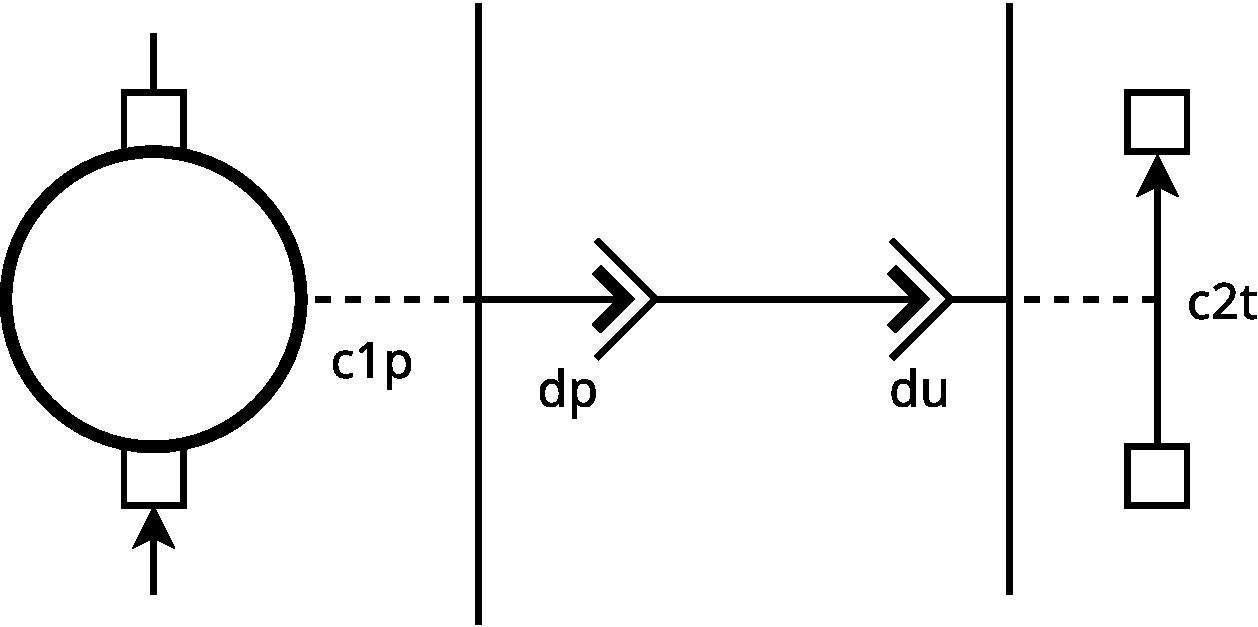
\includegraphics[scale=0.2]{images/perf_data_ports.pdf}
    \end{minipage}
  }
  \subfloat[Dependency graph]{%
    \begin{minipage}[c]{1.4\columnwidth}%
      \centering
      \begin{tikzpicture}[node distance=1.7cm]
        \node (c1t2) [beginning] {$v_\text{c1t2}^\text{beginning}$};
        \node (c1p1l) [leaving, below of=c1t2] {$v_\text{c1p}^\text{leaving}$};
        \node (c1p1) [place, below of=c1p1l] {$v_\text{c1p}^\text{place}$};
        \node (c1t1_end) [end, below of=c1p1] {$v_\text{c1t1}^\text{end}$};
        \draw [arrow] (c1t1_end) -- (c1p1) node[midway, right] {$0$};
        \draw [arrow] (c1p1) -- (c1p1l) node[midway, right] {$0$};
        \draw [arrow] (c1p1l) -- (c1t2) node[midway, right] {$0$};
        \node (dp) [provide_start, right of=c1p1, xshift=1.2cm] {$v_\text{dp}^\text{start}$};
        \node (du) [use_start, right of=dp, xshift=1.2cm] {$v_\text{du}^\text{start}$};
        \node (c2t) [beginning, right of=du, xshift=1.2cm] {$v_\text{c2t}^\text{beginning}$};
        \node (c2t_end) [end, above of=c2t] {$v_\text{c2t}^\text{end}$};
        \draw [arrow] (c2t) -- (c2t_end) node[midway, right] {$time(\text{c2t})$};
        \draw [arrow] (c1p1) -- (dp) node[midway, below] {$0$};
        \draw [arrow] (dp) -- (du) node[midway, below] {$0$};
        \draw [arrow] (du) -- (c2t) node[midway, below] {$0$};
      \end{tikzpicture}
    \end{minipage}
  }
  \caption{Vertices and arcs for data ports, bindings and connections}
  \label{fig:data_ports_graph}
\end{figure*}

For each connection between service provide port $p$ and service use port
$u$ in the assembly, we associate two arcs. The first from
$v_p^\text{start}$ to $v_u^\text{start}$ represents the fact that the
service may only be used after it has started being provided.
The second from $v_u^\text{stop}$ to $v_p^\text{stop}$ represents the fact
that the service may stop being provided only after it has stopped being
used.
Figure~\ref{fig:service_ports_graph} depicts the transformation of a
connection between service provide port \emph{sp} and service use port
\emph{su}.
\[
A_{L_{P}}=\bigcup_{\left(p,u\right)\in L_{P}}\left\{ \left(v_p^\text{start},v_u^\text{start},0\right),\left(v_u^\text{stop},v_p^\text{stop},0\right)\right\} 
\]

\begin{figure*}[h]
  \subfloat[Concerto assembly]{%
    \begin{minipage}[c]{0.7\columnwidth}%
      \centering
      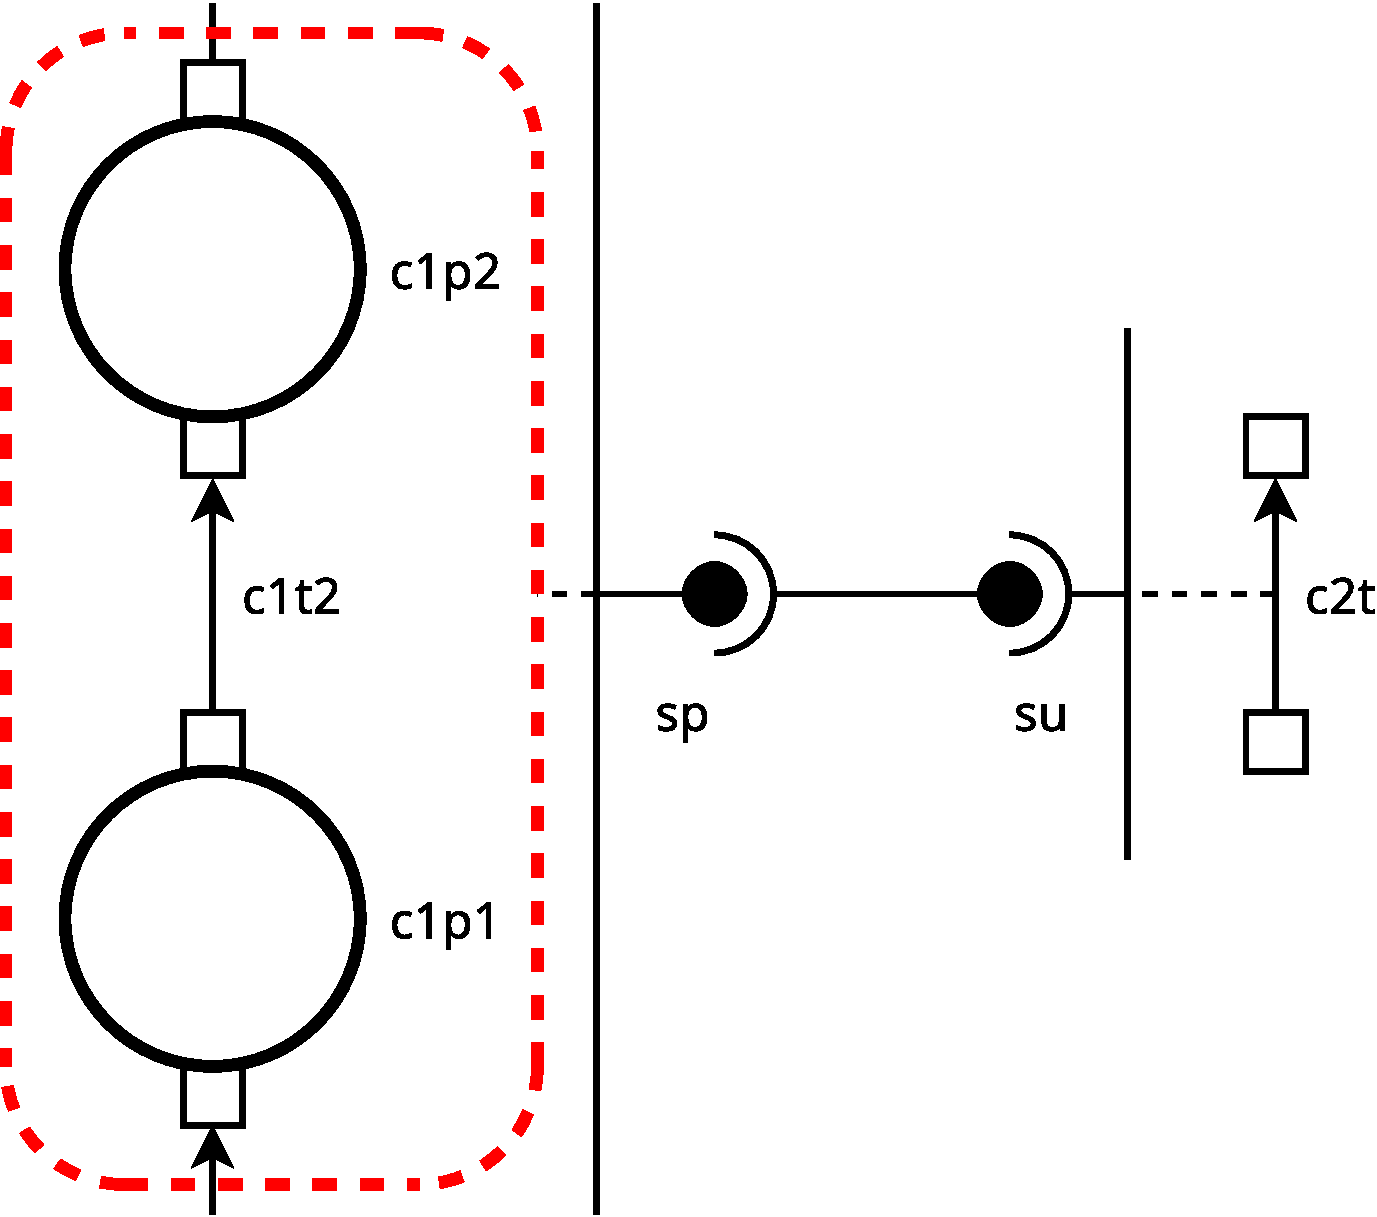
\includegraphics[scale=0.2]{images/perf_service_ports.pdf}
    \end{minipage}
  }
  \subfloat[Dependency graph]{%
    \begin{minipage}[c]{1.3\columnwidth}%
      \centering
      \begin{tikzpicture}[node distance=1.7cm]
        \node (c1t3) [beginning] {$v_\text{c1t3}^\text{beginning}$};
        \node (c1p2l) [leaving, below of=c1t3] {$v_\text{c1p2}^\text{leaving}$};
        \node (c1p2) [place, below of=c1p2l] {$v_\text{c1p2}^\text{place}$};
        \node (c1t2_end) [end, below of=c1p2] {$v_\text{c1t2}^\text{end}$};
        \node (c1t2) [beginning, below of=c1t2_end] {$v_\text{c1t2}^\text{beginning}$};
        \node (c1p1l) [leaving, below of=c1t2] {$v_\text{c1p1}^\text{leaving}$};
        \node (c1p1) [place, below of=c1p1l] {$v_\text{c1p1}^\text{place}$};
        \node (c1t1_end) [end, below of=c1p1] {$v_\text{c1t1}^\text{end}$};
        \draw [arrow] (c1t1_end) -- (c1p1) node[midway, right] {$0$};
        \draw [arrow] (c1p1) -- (c1p1l) node[midway, right] {$0$};
        \draw [arrow] (c1p1l) -- (c1t2) node[midway, right] {$0$};
        \draw [arrow] (c1t2) -- (c1t2_end) node[midway, right] {$time(\text{c1t2})$};
        \draw [arrow] (c1t2_end) -- (c1p2) node[midway, right] {$0$};
        \draw [arrow] (c1p2) -- (c1p2l) node[midway, right] {$0$};
        \draw [arrow] (c1p2l) -- (c1t3) node[midway, right] {$0$};
        \node (sp) [provide_start, right of=c1p1, xshift=1cm] {$v_\text{sp}^\text{start}$};
        \node (su) [use_start, right of=sp, xshift=1cm] {$v_\text{su}^\text{start}$};
        \node (c2t) [beginning, right of=su, xshift=1cm] {$v_\text{c2t}^\text{beginning}$};
        \node (c2t_end) [end, above of=c2t] {$v_\text{c2t}^\text{end}$};
        \node (sps) [provide_stop, right of=c1p2l, xshift=1cm] {$v_\text{sp}^\text{stop}$};
        \node (sus) [use_stop, left of=c2t_end, xshift=-1cm] {$v_\text{su}^\text{stop}$};
        \draw [arrow] (c2t) -- (c2t_end) node[midway, right] {$time(\text{c2t})$};
        \draw [arrow] (c1p1) -- (sp) node[midway, below] {$0$};
        \draw [arrow] (sp) -- (su) node[midway, below] {$0$};
        \draw [arrow] (su) -- (c2t) node[midway, below] {$0$};
        \draw [arrow] (c2t_end) -- (sus) node[midway, above] {$0$};
        \draw [arrow] (sus) -- (sps) node[midway, right] {$0$};
        \draw [arrow] (sps) -- (c1p2l) node[midway, above] {$0$};
      \end{tikzpicture}
    \end{minipage}
  }
  \caption{Vertices and arcs for service ports, bindings and connections}
  \label{fig:service_ports_graph}
\end{figure*}

For each initial place $\pi$ we associate one arc going from $v^\text{source}$
 to $v_\pi^\text{place}$, representing the fact that a token is placed in each
 initial place at the very beginning.
Figure~\ref{fig:source_sink_graph} depicts the transformation of two initial
places \emph{c1p1} and \emph{c2p2}.
\[
A_{I}=\bigcup_{\pi\in I_{all}}\left\{ \left(v^\text{source},v_\pi^\text{place},0\right)\right\} 
\]

In addition to the set of all initial places $I_{all}$, we define
the set of all final places $F_{all}$ as the set of places which
do not have any outgoing transition. Formally,
$F_{all}=\left\{ \pi\,\mid\,\pi\in\Pi_{all}\land\lnot\left(\exists\pi_{a}\in\Pi_{all}\,:\,\left(\pi,\pi_{a}\right)\in\Theta_{all}\right)\right\} $.
Then, for each final place $\pi$ we associate one arc going from
$v_\pi^\text{place}$ to $v^\text{sink}$, representing the fact that the
deployment is over only after all components have reached their final places
(\ie when no more transition can be executed).
Figure~\ref{fig:source_sink_graph} depicts the transformation of three final
places \emph{c1p2}, \emph{c2p2} and \emph{c2p3}.
\[
A_{F}=\left\{ v_\pi^\text{place},v^\text{sink},0\right\} 
\]

\begin{figure*}[h]
  \subfloat[Concerto assembly]{%
    \begin{minipage}[c]{0.7\columnwidth}%
      \centering
      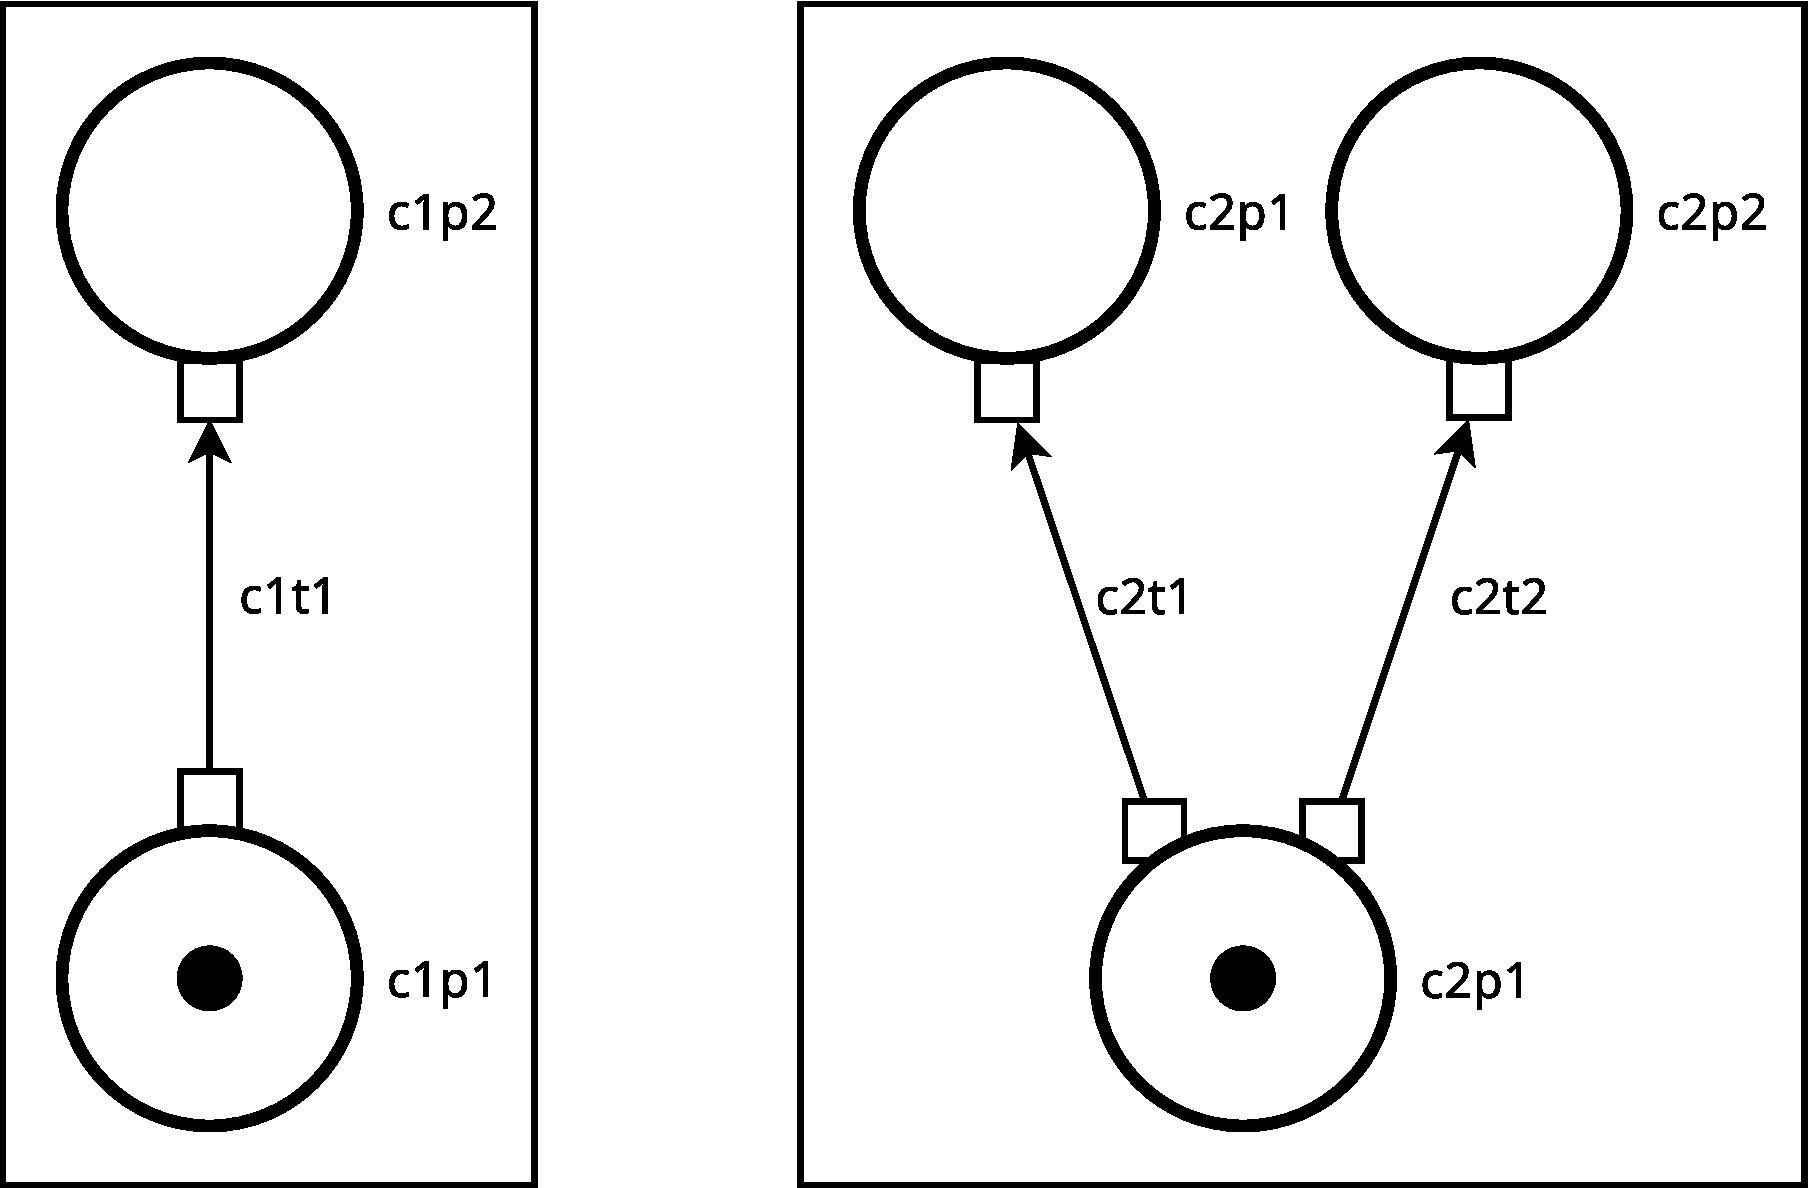
\includegraphics[scale=0.2]{images/perf_source_sink.pdf}
    \end{minipage}
  }
  \hfill
  \subfloat[Dependency graph]{%
    \begin{minipage}[c]{1.3\columnwidth}%
      \centering
      \begin{tikzpicture}[node distance=1.7cm]
        \node (c1p2l) [leaving] {$v_\text{c1p2}^\text{leaving}$};
        \node (c1p2) [place, below of=c1p2l,yshift=-0.3cm] {$v_\text{p1p2}^\text{place}$};
        \node (c1t1e) [end, below of=c1p2] {$v_\text{c1t1}^\text{end}$};
        \node (c1t1) [beginning, below of=c1t1e] {$v_\text{c1t1}^\text{beginning}$};
        \node (c1p1l) [leaving, below of=c1t1] {$v_\text{c1p1}^\text{leaving}$};
        \node (c1p1) [place, below of=c1p1l] {$v_\text{c1p1}^\text{place}$};
        
        \node (c2p2l) [leaving, right of=c1p2l, xshift=0.6cm, yshift=-0.6cm] {$v_\text{c2p2}^\text{leaving}$};
        \node (c2p2) [place, right of=c1p2, xshift=1.3cm] {$v_\text{c2p2}^\text{place}$};
        \node (c2t1e) [end, below of=c2p2] {$v_\text{c2t1}^\text{end}$};
        \node (c2t1) [beginning, below of=c2t1e] {$v_\text{c2t1}^\text{beginning}$};
        \node (c2p1l) [leaving, below of=c2t1, xshift=1.5cm] {$v_\text{c2p1}^\text{leaving}$};
        \node (c2p1) [place, below of=c2p1l] {$v_\text{c2p1}^\text{place}$};
        
        \node (c2p3) [place, right of=c2p2, xshift=1.3cm] {$v_\text{c2p3}^\text{place}$};
        \node (c2p3l) [leaving, above of=c2p3, yshift=0.3cm] {$v_\text{c2p3}^\text{leaving}$};
        \node (c2t2e) [end, below of=c2p3] {$v_\text{c2t2}^\text{end}$};
        \node (c2t2) [beginning, below of=c2t2e] {$v_\text{c2t2}^\text{beginning}$};
        
        \node (source) [control, below of=c2p1, xshift=-1.5cm] {$v^\text{source}$};
        \node (sink) [control, above of=c1p2l, xshift=3cm, yshift=0.6cm] {$v^\text{sink}$};
        
        \draw [arrow] (c1p1) -- (c1p1l) node[midway, right] {$0$};
        \draw [arrow] (c1p2) -- (c1p2l) node[midway, right] {$0$};
        \draw [arrow] (c2p1) -- (c2p1l) node[midway, right] {$0$};
        \draw [arrow] (c2p2) -- (c2p2l) node[midway, right] {$0$};
        \draw [arrow] (c2p3) -- (c2p3l) node[midway, right] {$0$};
        \draw [arrow] (c1t1) -- (c1t1e) node[midway, right] {$time(\text{c1t1})$};
        \draw [arrow] (c2t1) -- (c2t1e) node[midway, right] {$time(\text{c2t1})$};
        \draw [arrow] (c2t2) -- (c2t2e) node[midway, right] {$time(\text{c2t2})$};
        \draw [arrow] (c1p1l) -- (c1t1) node[midway, right] {$0$};
        \draw [arrow] (c2p1l) -- (c2t1) node[midway, right] {$0$};
        \draw [arrow] (c2p1l) -- (c2t2) node[midway, right] {$0$};
        \draw [arrow] (c1t1e) -- (c1p2) node[midway, right] {$0$};
        \draw [arrow] (c2t1e) -- (c2p2) node[midway, right] {$0$};
        \draw [arrow] (c2t2e) -- (c2p3) node[midway, right] {$0$};
        \draw [arrow] (source) -- (c1p1) node[midway, right] {$0$};
        \draw [arrow] (source) -- (c2p1) node[midway, right] {$0$};
        \draw [arrow] (c1p2) -- (sink) node[midway, right] {$0$};
        \draw [arrow] (c2p2) -- (sink) node[midway, right] {$0$};
        \draw [arrow] (c2p3) -- (sink) node[midway, right] {$0$};
      \end{tikzpicture}
    \end{minipage}
  }
  \caption{Arcs from source to initial places and from final places to sink. For the sake of clarity, there are no dependencies between the two components.}
  \label{fig:source_sink_graph}
\end{figure*}

Finally, we define $A$ as the union of all of these. 
\[
A=A_\Pi\cup A_{\Theta}\cup A_{D_{u}}\cup A_{D_{p}}\cup A_{P_{u}}\cup A_{P_{p}}\cup A_{L_{D}}\cup A_{L_{P}}\cup A_{I}\cup A_{F}
\]


\subsection{Time estimation}

We define the time estimation of the execution of the Madeus assembly
to be the length of the longest path between $v^\text{source}$ and
$v^\text{sink}$ in $G$. This path exists and is finite if $v^\text{sink}$ 
is reachable from $v^\text{source}$ and $G$ has no cycle.

Because the end of the execution of a Madeus component is defined as
when all its tokens are in final places, \ie there are no more transitions
to perform, the final places are necessarily connected to the initial place
in the \net. Because the dependency graph of the component keeps the same
shape as the \net, $v_{\pi_i}^\text{place}$ (where $\pi_i$ is the initial
place) is connected to all $v_{\pi_f}^\text{place}$ (where $\pi_f$ is a
final place). Because we connect $v^\text{source}$ to all
$v_{\pi_i}^\text{place}$ (where $v_{\pi_i}$ is the initial place of a
component) and all $v_{\pi_f}^\text{place}$ (where $\pi_f$ is a final place
of a component) to $v^\text{sink}$, there exists at least one path between
$v^\text{source}$ and $v^\text{sink}$ for each component. Therefore
$v^\text{sink}$ is reachable from $v^\text{source}$.

The dependency graph of each component has no cycle because it has the same
shape as the \net, in which there can be no cycle. Under some restriction
essentially preventing non-determinism, the arcs between the vertices
corresponding to port do not create cycles either. This restriction limits
the number of activation and deactivation of each port to one during the
deployment process. If there is no deadlock in the Madeus assembly, then
there can be no ``crossing dependencies'' (see Figure~\ref{fig:deadlock}). This means that
the activation and deactivation of two distinct sets of use and provide
ports cannot create a cycle. This reasoning also applies to the activation
and deactivation of a service use port and a service provide port. If they
were to happen in a different order in the two components, the dependency
graph would have a cycle, but because each port can be activated only once,
there would be a deadlock in the assembly.

\begin{figure}[h]
  \begin{center}
    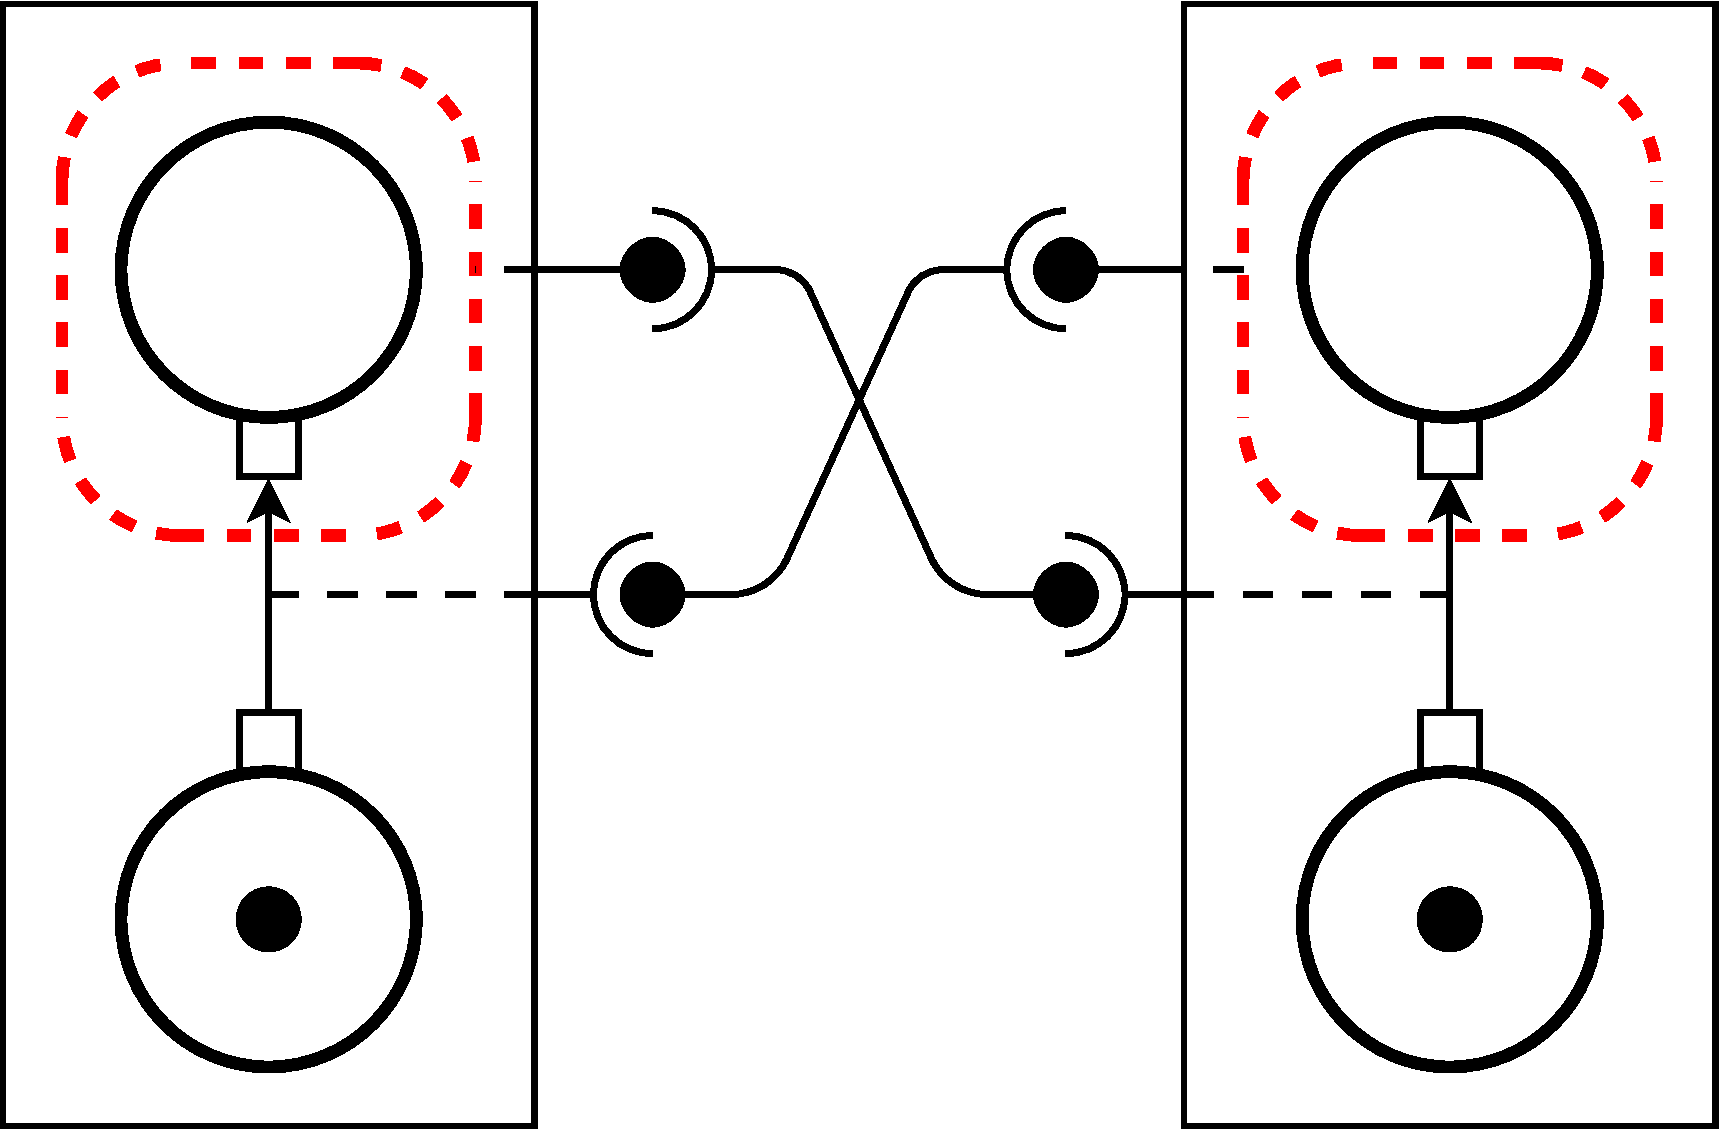
\includegraphics[width=0.7\linewidth]{./images/deadlock.pdf}
  \end{center}
  \caption{Example of an invalid assembly: crossing dependencies cause a deadlock.}
  \label{fig:deadlock}
\end{figure}

Because $G$ is a DAG, finding the longest path between $v^\text{source}$
and $v^\text{sink}$ can be done in $\mathcal{O}(|V|+|A|)$ by sorting the
vertices topologically and iterating through them, computing their maximum
distance from the source using the one of their parents. Note that
$|V| = \mathcal{O}(pl+tr+po)$ and $|A| = \mathcal{O}(tr+po+dp)$ where $pl$
is the number of places in the whole assembly, $tr$ is the number of
transitions, $po$ is the number of ports and $dp$ is the number of
dependencies. Therefore, the complexity of estimating the running time of
a Madeus deployment is $\mathcal{O}(pl+tr+po+dp)$.


\subsection{Requirements on the assembly}

In order to avoid non-determinism, which a dependency graph would not be
able to capture, we impose some requirements on a Madeus assembly
for it to be compatible with the performance model. However, these
requirements are quite reasonable in the sense that none of the use
cases we have thought of do not meet these requirements.
%
First, each port may only be activated once and deactivated once, and
may only be connected to one group. Second, all groups must have a
single entry point, \ie only one transition going from a place outside
of the group to a place inside of the group. Likewise, they must have a
single exit point (if any), \ie at most one transition going from a
place inside of the group to a place outside of the group.

\subsection{Example}

\MC[Hélène]{Prendrait trop de place ? (vu la taille de la Figure~\ref{fig:source_sink_graph})}
